\documentclass[a4paper,12pt]{article}
\usepackage[utf8x]{inputenc}
\usepackage{amssymb}
\usepackage{amsfonts}
\usepackage{mathrsfs}
\usepackage{amsmath}
\usepackage{amsthm}
\usepackage[margin=3cm]{geometry}
\usepackage{times}
\usepackage{graphicx}
\usepackage{enumitem}
\usepackage{fancyhdr}
\usepackage{hyperref}
\usepackage{setspace}
\usepackage{subcaption}
\usepackage{mathtools}

\pagestyle{fancy}
\fancyhf{}
\lhead{Thomas Delaney}
\rhead{Communities in correlation based networks}
\cfoot{\thepage}

\newtheorem{theorem}{Theorem}
\newtheorem{proposition}{Proposition}[section]
\newtheorem{lemma}{Lemma}[section]
\newtheorem{corollary}{Corollary}[section]
\theoremstyle{definition}
\newtheorem{definition}{Definition}[section]

\newcommand{\boldnabla}{\mbox{\boldmath$\nabla$}} % to be used in mathmode
\newcommand{\cbar}{\overline{\mathbb{C}}}% to be used in mathmode
\newcommand{\diff}[2]{\frac{d #1}{d #2}}% to be used in mathmode
\newcommand{\difff}[2]{\frac{d^2 #1}{d #2^2}}% to be used in mathmode
\newcommand{\pdiff}[2]{\frac{\partial #1}{\partial #2}} % to be used in mathmode
\newcommand{\pdifff}[2]{\frac{\partial^2 #1}{\partial #2^2}}% to be used in mathmode
\newcommand{\upperth}{$^{\mbox{\footnotesize{th}}}$}%to be used in text mode
\newcommand{\vect}[1]{\mathbf{#1}}% to be used in mathmode
\newcommand{\curl}[1]{\boldnabla \times \vect{#1}} % to be used in mathmode
\newcommand{\divr}[1]{\boldnabla \cdot \vect{#1}} %to be used in mathmode
\newcommand{\modu}[1]{\left| #1 \right|} %to be used in mathmode
\newcommand{\brak}[1]{\left( #1 \right)} % to be used in mathmode
\newcommand{\comm}[2]{\left[ #1 , #2 \right]} %to be used in mathmode
\newcommand{\dop}{\vect{d}} %to be used in mathmode
\newcommand{\cov}{\text{cov}} %to be used in mathmode
\newcommand{\var}{\text{var}} %to be used in mathmode
\newcommand{\mb}{\mathbf} %to be used in mathmode
\newcommand{\bs}{\boldsymbol} %to be used in mathmode
% Title Page
\title{Communities in correlation based networks}
\author{Thomas Delaney}

\begin{document}

\tableofcontents

\newpage

\section{Motivation}
    \subsection{Finding highly correlated networks including cells from different anatomical regions}
    Decades of research has established that these correlations play a crucial role in representing sensory information. For example, the onset of visual attention has been shown to have a greater affect on the correlations in the macaque V4 than on the firing rates in that region \cite{cohen1}. Recent findings show that spontaneous behaviours explain correlations in parts of the brain not associated with motor control \cite{stringer}. In order to understand the brain, we must understand the interactions between neurons. 

    Because of limitations in recording technology almost all research has explored correlations between neurons within a given brain region. Relatively little is known about correlations between neurons in different brain regions. However, the recent development of `Neuropixels' probes \cite{jun} has allowed extracellular voltage measurements to be collected from multiple brain regions simultaneously routinely, and in much larger numbers than traditional methods. In this project we used a publicly-available Neuropixels dataset to analyse correlations between different brain regions \cite{stringer}.

    We wanted to find highly correlated communities among larger ensembles of neurons, including neurons from different anatomical regions. In order to do this, we induced an undirected weighted network in the neural ensemble by measuring the spike count correlations between every pair of neurons. We then used a cutting edge community detection method \cite{humphries} on this network to find any highly correlated communities present in the ensemble. We also treated the anatomical regions and the detected communities as clusterings of cells, and used clustering comparison methods to measure how different these clusterings were.

    \subsection{Changing timescales}
    The time bin width used when binning spike trains into spike counts affects spike count correlation measures \cite{cohen2}. We explored the effect of changing time bin width on the correlations between neurons. In doing so, we noticed that \textit{within-region} correlations were affected differently to \textit{between-region} correlations. In order to quantify these differences, we measured the correlations and carried out the community detection, and the clustering comparison using different values for the time bin width. 
    
% we're getting into results here Need more motivation.

\section{Data}
    \subsection{Brain regions}
    Neuropixels probes were used to collect extracellular recordings \cite{jun} from three different mice. The mice were awake and enganging in spontaneous behaviour. 
    \begin{enumerate}
        \item male, wild type, P73. % Robbins
        \item female, TetO-GCaMP6s, Camk2a-tTa, P113 % Waksman
        \item male, Ai32, Pvalb-Cre, P99 % Krebs
    \end{enumerate}
    Eight probes were used to collect readings from 2296, 2668, and 1462 cells respectively. Data were collected from nine brain regions in each mouse:
    \begin{itemize}
        \item Caudate Putamen (CP)
        \item Frontal Motor Cortex (Frmoctx)
        \item Hippocampal formation (Hpf)
        \item Lateral Septum (Ls)
        \item Midbrain (Mb)
        \item Superior Colliculus (Sc)
        \item Somatomotor cortex (Sommoctx)
        \item Thalamus (Th)
        \item Primary visual cortex (V1)
    \end{itemize}
    Readings were continuous and lasted for about 1 hour \cite{stringer}.

    \subsection{Video recordings}\label{sec:video_recordings}
    Video recordings of the mouse's face were taken during the spontaneous behaviour. We had access to the top $500$ principle components and top $500$ eigenvectors of the processed video. The frequency of recording was slightly less than $40$Hz. Recordings were $327 \times 561$ pixels. These principal components were used as behavioural data. We controlled for these components when taking measurements conditional on behaviour. 

\section{Methods}
    \subsection{Binning data}
    The data were divided into time bins of various widths ranging from $0.01$s to $4$s. If the total length of the recording period was not an integer multiple of the time bin width, we cut off the remaining time at the end of the recording period. This period was at most $3.99$s. This is far less than the total recording time of around $1$ hour.

    \subsection{Correlation coefficients}
    We calculated Pearson's correlation coefficient for pairs of neurons. For jointly distributed random variables $X$ and $Y$, Pearson's correlation coefficient is defined as:
    \begin{align}\label{eq:dist_pearsons_corr}
        \rho_{XY} =& \frac{\cov(X,Y)}{\sigma_X \sigma_Y} \\
                  =& \frac{E[(X - \mu_X)(Y - \mu_Y)]}{\sigma_X \sigma_Y}
    \end{align}
    where $E$ denotes the expected value, $\mu$ denotes the mean, and $\sigma$ denotes the standard deviation. The correlation coefficient is a normalised measure of the covariance. It can take values between $1$ (completely correlated) and $-1$ (completely anti-correlated). Two independent variables will have a correlation coefficient of $0$. But, having $0$ correlation does not imply independence.

    If we do not know the means and standard deviations required for equation \ref{eq:dist_pearsons_corr}, but we have samples from $X$ and $Y$, Pearson's sample correlation coefficient is defined as:
    \begin{align}
        r_{XY} = \frac{\sum_{i=1}^n (x_i - \bar{x})(y_i - \bar{y})}{\sqrt{\sum_{i=1}^n (x_i - \bar{x})^2}\sqrt{\sum_{i=1}^n (y_i - \bar{y})^2}}
    \end{align}
    where $\lbrace (x_i, y_i) \rbrace$ for $i \in \lbrace 1, \dots, n \rbrace$ are the paired samples from $X$ and $Y$, and $\bar{x} = \frac{1}{n}\sum_{i=1}^n x_i$, and $\bar{y} = \frac{1}{n}\sum_{i=1}^n y_i$ are the sample means.

    In practice we used the python function \texttt{scipy.stats.pearsonr} to calculate the correlation coefficients.

        \subsubsection{Spike Count Correlation, $r_{SC}$}\label{sec:spike_count_correlation}
        The spike count correlation ($r_{SC}$) of two cells is the correlation between the spike counts of those cells in response to a given stimulus condition. In this study, there was only one stimulus condition, that of no stimulus. The subjects engaged in spontaneous behaviour during recording.

        \subsubsection{Shuffled spike count correlations}
        We measured the shuffled spike count correlations between two neurons by randomly permuting one of the neuron's spike counts and measuring the spike count correlations. These shuffled correlations were useful when measuring the effect of time bin width on correlations, and when deciding which correlations should be preserved when creating correlation networks (see section \ref{sec:sparsifying_data_networks}). 

        \subsubsection{Separating Correlations \& Anti-correlations}\label{sec:corr_anti_corr} 
        In order to compare the effect of bin width on measures of negative $r_{SC}$ (anti-correlation) and positive $r_{SC}$ separately, we had to separate correlated and anti-correlated pairs. To do this, we simply measured the mean $r_{SC}$, taking the mean across all the bin widths. If this quantity was positive or zero we regarded the pair as positively correlated. If this quantity was negative we regarded the pair as anti-correlated.

    \subsection{Conditioning on behavioural data}
    Our behavioural data consisted of the top $500$ principal components (PCs) of a processed video recording of the mouse's face (see section \ref{sec:video_recordings}). Denoting the spike count of a given cell by $X$, and the PCs by $Z_1,\dots,Z_{500}$, we wanted to model $X$ as a function of $Z_1,\dots,Z_{500}$ in order to estimate
    \begin{align}
      E[X|Z_1,\dots,Z_{500}] &= \int_{x \in X} x P(X=x | Z_1,\dots,Z_{500}) dx \\
        &= \int_{x \in X} x \frac{P(X=x, Z_1,\dots,Z_{500})}{P(Z_1,\dots,Z_{500})} dx
    \end{align}
    Given the $500$ components, a na\"{i}ve estimation of $P(Z_1,\dots,Z_{500})$ or $P(X, Z_1,\dots,Z_{500})$ by histogramming was impossible. Therefore we modelled $X$ as a linear combination of the PCs.

        \subsubsection{Linear regression}
        We modelled the spike count of a given cell, $X$, as a linear combination of the PCs of the video of the mouse's face, $\mathbf{Z} = Z_1,\dots,Z_{500}$. We tried three different types of regularization 
        \begin{itemize}
            \item $L1$ or `Lasso'
            \item $L2$ or `Ridge regression'
            \item `Elastic net' regularisation (a linear combination of both $L1$ and $L2$ regularisation penalities)
        \end{itemize}
        The elastic net regularisation performed the best, so we stuck with that.

        \subsubsection{Elastic net regularisation}
        Suppose we wish to model $n$ observations of a random variable $X$, $\mathbf{x} = (x_1, \cdots, x_n)$ using $n$ instances of $m$ predictors $\mathbf{Z} = (Z_1, \cdots, Z_m)$. The na\"{i}ve elastic net criterion is
        \begin{align}\label{eq:elastic_net}
            L(\lambda_1, \lambda_2, \boldsymbol{\beta}) = | \mathbf{x} - \mathbf{Z} \boldsymbol{\beta} |^2 + \lambda_2 |\boldsymbol{\beta}|_2 + \lambda_1 |\boldsymbol{\beta}|_1
        \end{align}
        where
        \begin{align}
          |\boldsymbol{\beta}|_2 &= \sum_{j=1}^m \beta_j^2 \\
          |\boldsymbol{\beta}|_1 &= \sum_{j=1}^m |\beta_j|
        \end{align}
        The na\"{i}ve elastic net estimator $\hat{\boldsymbol{\beta}}$ is the minimiser of the system of equations \ref{eq:elastic_net} \cite{zou}
        \begin{align}
          \hat{\boldsymbol{\beta}} = \arg \min_{\boldsymbol{\beta}} L(\lambda_1, \lambda_2, \boldsymbol{\beta})
        \end{align}
        We implemented the model using the \texttt{ElasticNetCV} method of Python's \\ \texttt{sklearn.linear\_models} package.

        As well as using the PCs, we also tried fitting the models using the raw video data reconstructed from the PCs and eigenvectors. These models performed worse than those using the PCs. We expected this because each representation contains the same amount of information, but the raw video representation spreads this information across many more components. This requires more parameter fitting, but given the same information. 

        \subsubsection{Conditional covariance}
        We calculated the expected value of the conditional covariance using the law of total covariance.
        \begin{align}\label{eq:law_of_total_covariance}
            \cov (X,Y) = E[ \cov(X,Y|Z)] + \cov(E[X|Z], E[Y|Z])
        \end{align}
        where these expected values are calculated with respect to the distribution of $Z$ as a random variable.

        Using our linear model, we calculated $E[X|Z_1,\dots, Z_{500}]$ for each cell $X$. Then we proceeded to calculate
        \begin{align}
            E[\cov(X,Y|Z_1,\dots, Z_{500})] = \cov(X,Y) - \cov(E[X|Z_1,\dots, Z_{500}], E[Y|Z_1,\dots, Z_{500}])
        \end{align}

        \subsubsection{Measures of conditional correlation}
        As a measure of expected correlation, we measured the `event conditional correlation' \cite{maugis}
        \begin{align}\label{eq:event_conditional_correlation}
            \rho_{XY|Z} = \frac{E[\cov(X,Y|Z)]}{\sqrt{E[\var(X|Z)]E[\var(Y|Z)]}}
        \end{align}
        (I need to read more about this. This is not really a correlation)

        For comparison, we also measured the `signal correlation'
        \begin{align}\label{eq:signal_correlation}
            \rho_{\text{signal}} = \frac{\cov(E[X|Z], E[Y|Z])}{\sqrt{\var(E[X|Z])\var(E[Y|Z])}}
        \end{align}
        this is an actual correlation, at least.
        

    \subsection{Information Theory}\label{sec:information_theory}
        \subsubsection{Entropy $H(X)$}
        The entropy of a random variable $X$, with outcomes $x_1, \dots, x_N$, and corresponding probabilities $p_1, \dots, p_N$ is defined as
        \begin{align}\label{entropy}
        H(X) = -\sum_{n=1}^N p_n \log _2 p_n
        \end{align}
        This quantity is also known as the information entropy or the `surprise'. It measures the amount of uncertainty in a random variable. For example, a variable with a probability of $1$ for one outcome, and $0$ for all other outcomes will have 0 bits entropy, because it contains no uncertainty. But a variable with a uniform distribution will have maximal entropy as it is the least predictable. This quantity is analogous to the entropy of a physical system \cite{shannon}. Note that any base may be used for the logarithm in equation \ref{entropy}, but using base $2$ means that the quantity will be measured in `bits'.

        The joint entropy of two jointly distributed random variables $X$ and $Y$, where $Y$ has outcomes $y_1, \dots, y_M$, is defined as
        \begin{align}\label{joint_entropy}
        H(X, Y) = -\sum_{n=1}^N \sum_{m=1}^M P(X=x_n, Y=y_m) \log _2 P(X=x_n, Y=y_m)
        \end{align}
        If $X$ and $Y$ are independent then $H(X,Y) = H(X) + H(Y)$. Otherwise $H(X,Y) < H(X) + H(Y)$. When $X$ and $Y$ and completely dependent $H(X,Y) = H(X) = H(Y)$.

        The conditional entropy of $Y$ conditioned on $X$ is defined as
        \begin{align}
        H(Y|X) = -\sum_{n=1}^N \sum_{m=1}^M P(X=x_n, Y=y_m) \log _2 \frac{P(X=x_n, Y=y_m)}{P(X=x_n)}
        \end{align}
        When $X$ and $Y$ are independent $H(Y|X) = H(Y)$. Intuitively, we learn nothing of $Y$ by knowing $X$, so $Y$ is equally uncertain whether we know $X$ or not. If $Y$ is totally dependent on $X$, then the fraction in the logarithm is $1$, which gives $H(Y|X) = 0$.

        These entropy measures are the basis of the mutual information measure.

        \subsubsection{Maximum entropy limit}\label{sec:entropy_limit}
        When spiking data is binned into spike counts there is an upper limit on the entropy of these data. The maximum entropy discrete distribution is the discrete uniform distribution. A random variable with this distribution will take values from some finite set with equal probabilities. Binned spike count data will take values between $0$ and some maximum observed spike count $n_{\max}$. A neuron with responses that maximises entropy will take these values with equal probability, i.e. if $i \in \lbrace 0, \dots, n_{\max} \rbrace$ then $P(X = i) = \frac{1}{n_{\max} + 1}$. The entropy of this neuron will be
        \begin{align*}
          H(X)  &= - \sum_{i=0}^{n_{\max}} P(X = i) \log _2 P(X=i) \\
                &= - \sum_{i=0}^{n_{\max}} \frac{1}{n_{\max} + 1} \log_2 \left( \frac{1}{n_{\max} + 1} \right) \\
                &= - \log_2 \left( \frac{1}{n_{\max} + 1} \right) \\
                &= \log_2 \left( n_{\max} + 1 \right)
        \end{align*}
        Therefore, the maximum entropy of the binned spike counts of a neuron is $\log _2 \left( n_{\max} + 1 \right)$. Of course, it would be very unusual for a neuron to fire in accordance with the discrete uniform distribution. Most measures of entropy taken on binned spiking data will be much lower than the maximum. See figure \ref{fig:entropy_limit} to see the maximum entropy as a function of the maximum observed spike count.

        \begin{figure}[h]
          \centering
          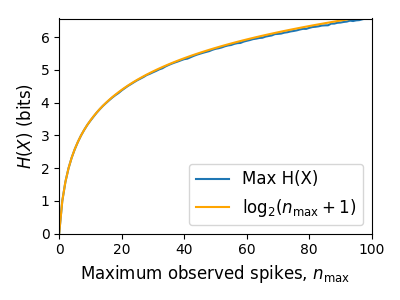
\includegraphics[width=0.5\textwidth]{figures/entropy_limit.png}
          \caption{\textbf{Entropy Limit:} The uppper limit on entropy of binned spike count data as a function of the maximum observed spike count. The orange line is the analytical maximum. The blue line is the entropy of samples with $N=1000$ data points taken from the discrete uniform distribution.}
          \label{fig:entropy_limit}
        \end{figure}

        \subsubsection{Mutual Information $I(X;Y)$}
        The mutual information can be defined mathematically in a number of ways, all of which are equivalent. These definitions illustrate the different ways of interpreting the mutual information.

        For two jointly distributed random variables $X$ and $Y$, the mutual information $I(X;Y)$ is defined as
        \begin{align}\label{eq:mutual_info_intuitive}
        I(X;Y)  =& H(Y) - H(Y|X) \\
                =& H(X) - H(X|Y)
        \end{align}
        Equation \ref{eq:mutual_info_intuitive} fits with the following intuition: The mutual information between $X$ and $Y$ is the reduction in uncertainty about $X$ gained by knowing $Y$, or vice versa. We could also say the mutual information is the amount of information gained about $X$ by knowing $Y$, or vice versa.

        Another useful entropy based definition for the mutual information is
        \begin{align}\label{eq:mutual_info_useful}
        I(X;Y)  =& H(X) + H(Y) - H(X,Y)
        \end{align}
        This definition is useful because it does not require the calculation of conditional probabilities. This was the form we used when performing calculations.

        The mutual information can also be defined in terms of marginal, joint, and conditional distributions. For example,
        \begin{align}\label{eq:mutual_info_log}
        I(X;Y)  =& -\sum_{n=1}^N \sum_{m=1}^M P(X=x_n, Y=y_m) \log _2 \frac{P(X=x_n, Y=y_m)}{P(X=x_n) P(Y=y_m)}
        \end{align}
        Notice that this can be rewritten as a Kullback–Leibler divergence.
        \begin{align}
        I(X;Y)  =& D_{KL}(P(X,Y)|| P(X)P(Y))
        \end{align}
        So, we can also think of the mutual information as a measure of the difference between the joint distribution of $X$ and $Y$, and the product of their marginal distributions. Since the product of the marginal distributions is the joint distribution for independent variables, we can think of the mutual information as a measure of the variables' dependence on one another.

        The minimum value that $I(X;Y)$ can take is $0$. This occurs when the random variables $X$ and $Y$ are independent. Then we have $H(X|Y) = H(X)$, and $H(Y|X) = H(Y)$, which according to equation \ref{eq:mutual_info_intuitive}, gives $I(X;Y) = 0$. We also have that $H(X,Y) = H(X) + H(Y)$ in this case, which according equation \ref{eq:mutual_info_useful}, gives $I(X;Y) = 0$. Finally, we also have $P(X,Y) = P(X)P(Y)$, which leaves us with $1$ in the argument for the logarithm in equation \ref{eq:mutual_info_log}, which again gives $I(X;Y) = 0$.

        The mutual information reaches its maximum value when one of the variables $X$ and $Y$ is completely determined by knowing the value of the other. In that case $I(X;Y) = \min \lbrace H(X), H(Y) \rbrace$.

        \subsubsection{Variation of Information $VI(X,Y)$}\label{sec:variation_of_information}
        The variation of information is another information theoretical quantity based on the mutual information. It is defined as
        \begin{align}\label{eq:variation_of_information}
            VI(X;Y) = H(X) + H(Y) - 2 I(X;Y)
        \end{align}
        We can rewrite this as the summation of two positive quantities
        \begin{align}
            VI(X;Y) = \left[ H(X) - I(X;Y) \right] + \left[ H(Y) - I(X;Y) \right]
        \end{align}
        In English, the variation of information is the summation of the uncertainty in the random variables $X$ and $Y$ excluding the uncertainty shared by those variables.

        This measure will become more relevant when we go on to talk about clusterings because $VI(X;Y)$ forms a metric on the space of clusterings.

        \subsubsection{Measuring entropies \& mutual information}
        In practice, we measured the mutual information between spike counts using Python and the python package \texttt{pyitlib}. We used the PT-bias correction technique to estimate the bias of our measurements when measuring the mutual information between the spike counts of two cells \cite{treves}.

        When measuring the mutual information between clusterings we used Python, but we used the \texttt{mutual\_info\_score}, \texttt{adjusted\_mutual\_info\_score}, and \texttt{normalized\_mutual\_info\_score} functions from the \texttt{sklearn.metrics} part of the \texttt{sklearn} package.

    \subsection{Network analysis}
        \subsubsection{Correlation networks}
        In order to analyse functional networks created by the neurons in our ensemble, we measured the spike count correlation between each pair of neurons. These measurements induced an undirected weighted network between the neurons. The weight of each connection was equal to the spike count correlation between each pair of neurons. 

        \subsubsection{Rectified correlations}
        At the time of writing, the community detection method outlined in \cite{humphries} could only be applied to networks with positively weighted connections. But many neuron pairs were negatively correlated. To apply the community detection method, we \textit{rectified} the network, by setting all the negative weights to zero.

        We also looked for structure in the network created by negative correlations by reversing the signs of the correlations, and rectifying these correlations before applying our network analysis.

        \subsubsection{Sparsifying data networks}\label{sec:sparsifying_data_networks}
        When creating our correlation networks, we wanted to exclude any correlations that could be judged to exist `by chance'. To do this, we measured the $5$th and $95$th percentile of the shuffled correlations for the given mouse and time bin width. We then set all the data correlations between these two values to $0$. This excluded any `chance' correlations from our network, and created a sparser network. 

        \subsubsection{Communities}
        Given some network represented by an adjacency matrix $\mathbf{A}$, a community within that network is defined as a collection of nodes where the number of connections within these nodes is higher than the expected number of connections between these nodes. In order to quantify the `expected' number of connections, we need a model of a community-less network. In the context of community detection, a community-less model is a network null model. We test the hypothesis that our data model departs from the community-less null model to a statistically significant degree. For undirected unweigted networks, the canonical model of a community-less network is the configuration model \cite{fosdick}. Since we are working with weighted sparse networks, we used more suitable null models, described below.

        \subsubsection{Weighted configuration model}\label{sec:weight_configuration_model}
        The \textit{weighted configuration model} is a canonical null network model for weighted networks. Given some data network, the weighted configuration model null network will preserve the degree sequence and weight sequence of each node in the data network. But the edges will be distributed randomly \cite{fosdick}. Any structure in the data network beyond its degree sequence and weight sequence will be removed in the weighted configuration model. So, this model can be used in testing the hypothesis that this extra structure exists. 

        \subsubsection{Sparse weighted configuration model}\label{sec:sparse_weighted_configuration_model}
        The \textit{sparse weighted configuration model} is another null network model. Similar in nature to the weighted configuration model (see section \ref{sec:weight_configuration_model}), but the sparsity of the data network is preserved in the null network. This is achieved by sampling from a probability distributon for the creation or non-creation of each possible connection, then distributing the weight of the data network randomly in this sparse network \cite{humphries}. This is the null network that we used when searching for additional strcuture in our data networks.

        \subsubsection{Spectral rejection}\label{sec:spectral_rejection}
        We made use of the spectral rejection algorithm as outlined in \cite{humphries}. The spectral rejection algorithm is a method for finding structure in a network not captured by a supposed null model, if such structure exists. 
        
        To describe the method, we denote our data network matrix $\mathbf{W}$, we denote the expected network of our null network model as $\left\langle \mathbf{P} \right\rangle$. Then the departure of our data network from the null network can be described by the matrix
        \begin{align}
          \mathbf{B} = \mathbf{W} - \left\langle \mathbf{P} \right\rangle
        \end{align}
        a common choice for $\left\langle \mathbf{P} \right\rangle$ in community detection is the `configuration model' \cite{fosdick, humphries2}. The matrix $\mathbf{B}$ is often called the configuration matrix, in this context we will use the term `deviation matrix' as it captures the deviation of $\mathbf{W}$ from the null model. 

        To test for structure in the network represented by $\mathbf{W}$, we examine the eigenspectrum of $\mathbf{B}$ and compare it to the eigenspectrum of our null model. Firstly, note that since our data model doesn't allow self loops, and is not directed, the matrix representing the network will be symmetric and positive semi-definite, and will therefore be invertible with real eigenvalues. We selected a null model with the same characteristics. 
        
        To find the eigenspectrum of the null model, we generated $N$ samples from our null model $P_1, \dots, P_N$, and we measured their deviation matrices $B_1, \dots, B_N$. We then calculated the eigenspectrum of each of those samples. We calculated the upper bound of the null model eigenspectrum by taking the mean of the largest eigenvalues of $B_1, \dots, B_N$. We calculated a lower bound on the null model eigenspectrum by taking the mean of the smallest eigenvalues of $B_1, \dots, B_N$. 

        We then calculated the eigenspectrum of $\mathbf{B}$, our data network deviation matrix. If any of those eigenvalues lay outside of the upper or lower bounds of the null model eigenspectrum, this is evidence of additional structure not captured by the null model. If we chose the sparse weighted configuration model (seec section \ref{sec:sparse_weighted_configuration_model}) as our null network model, then eigenvalues lying below the lower bound indicate $n$-partite structure in the network. For example, if one eigenvalue lay below the lower bound, this would indicate some bipartite structure in the data network. If any eigenvalues lay above the upper bound of the null model eigenspectrum, this is evidence of community structure in the data network. For example, one eigenvalue of $\mathbf{B}$ lying above the upper bound of the null model eigenspectrum indicates the presence of two communities in the network \cite{humphries2}.

        \subsubsection{Node rejection}
        If there are $d$ data eigenvalues lying outside of the null network eigenspectrum, the $d$ eigenvectors corresponding to these eigenvalues will form a vector space. If we project the nodes of our network into this vector space, by projecting either rows or colmns of the data matrix, we can see how strongly each node contributes to the vector space. Nodes that contribute strongly to the additional structure will project far away from the origin, nodes that do not contribute to the additional structure will project close to the origin. We want to use this information to discard those nodes that do not contribute.

        We can test whether a node projects \textit{far} away from the origin or \textit{close} to the origin using the eigenvalues and eigenvectors of $B_1, \dots, B_N$. The $j$th eigenvector and eigenvalue of $B_i$ gives a value for a null network's projection into the $j$th dimension of the additional structure vector space. The matrices $B_1, \dots, B_N$ give $N$ projections into that dimension. These projections are a distribution of null networks' projections. If the data node's projection exceeds that of the null network projections this node is judged to project \textit{far} from the origin, and therefore contribute to the additional structure. Otherwise, the node is judged to project \textit{close} to the origin, and is therefore rejected \cite{humphries}.

        \subsubsection{Community detection}
        Another application for this $d$ dimensional space is community detection. We first project all of the nodes into this $d$-dimensional space, then perform the clustering in this space. The clustering and community detection procedure is described in \cite{humphries2}. 

        In practice, the procedure is carried out $n$ times (we chose $n=100$ times), this returns $n$ clusterings. We resolve these $n$ clusterings to one final clustering using \textit{consensus clustering}. We used the consensus clustering method that uses an explicit null model for the consensus matrix, as outlined in \cite{humphries}.

    \subsection{Clustering Comparison}
    A clustering $\mathcal{C}$ is a partition of a set $D$ into sets $C_1, C_2, \dots, C_K$, called clusters, that satisfy the following for all $k,l \in \lbrace 1,\dots,K \rbrace$:
    \begin{align}
        C_k \cap C_l &= \emptyset \\
        \bigcup_{k=1}^K C_k &= D
    \end{align}
    If we consider two clusterings, $\mathcal{C}$ with clusters $C_1, C_2, \dots, C_K$ and $\mathcal{C}^{\prime}$ with clusters $C_1^{\prime}, C_2^{\prime}, \dots, C_K^{\prime}$. There are a number of measurements we can use to compare $\mathcal{C}$ and $\mathcal{C}^{\prime}$. In the following, the number of elements in $D$ is denoted by $n$, and the number of elements in cluster $C_k$ is $n_k$.

      \subsubsection{Adjusted Rand Index}
      The \textit{adjusted Rand Index} is a normalised similarity measure for clusterings based on pair counting.

      If we consider the clusterings $\mathcal{C}$ and $\mathcal{C}^{\prime}$, and denote
      \begin{itemize}
        \item the number of pairs in the same cluster in $\mathcal{C}$ and $\mathcal{C}^{\prime}$ by $N_{11}$
        \item the number of pairs in different clusters in $\mathcal{C}$ and $\mathcal{C}^{\prime}$ by $N_{00}$
        \item the number of pairs in the same cluster in $\mathcal{C}$ and different clusters in $\mathcal{C}^{\prime}$ by $N_{10}$
        \item the number of pairs in different clusters in $\mathcal{C}$ and the same cluster in $\mathcal{C}^{\prime}$ by $N_{01}$
      \end{itemize}
      then the \textit{Rand Index} is defined as 
      \begin{align}
          RI = \frac{N_{11} + N_{00}}{N_{11} + N_{00} + N_{10} + N_{01}} = \frac{N_{11} + N_{00}}{\binom{n}{2}}
      \end{align}
      The Rand Index is $1$ when the clusterings are identical, and $0$ when the clusterings are completely different.

      The \textit{adjusted Rand Index} intends on correcting the Rand Index for chance matching pairs. This is defined as 
      \begin{align}
          ARI = \frac{2\left( N_{00}N_{11} - N_{01}N_{10} \right)}{\left( N_{00} + N_{01} \right)\left( N_{01} + N_{11} \right) + \left( N_{00} + N_{10} \right)\left( N_{10} + N_{11} \right)}
      \end{align}
      The adjusted Rand Index is $1$ when the clusterings are identical, and $0$ when the Rand Index is equal to its expected value.

      \subsubsection{Clusterings as random variables}
      If we take any random element of $D$, the probability that this element is in cluster $C_k$ of clustering $\mathcal{C}$ is 
      \begin{align}
          P(K=k) = \frac{n_k}{n}
      \end{align}
      this defines a probability distribution, which makes the clustering a random variable. Any clustering can be considered as a random variable this way. 

      This means that we can measure any of the information theoretic quantities defined in section \ref{sec:information_theory} with respect to clusterings. For example, the entropy of a clustering is 
      \begin{align}
          H(\mathcal{C}) = - \sum_{k=1}^K \frac{n_k}{n} \log \frac{n_k}{n}
      \end{align}
      If we have two clusterings, the joint probability distribution of these clusterings is defined as
      \begin{align}
          P(K=k,K^{\prime}=k^{\prime}) = \frac{|C_k \cap C^{\prime}_{k^\prime}|}{n}
      \end{align}
      The joint distribution allows us to define the mutual information between two clusterings, $I(\mathcal{C};\mathcal{C}^{\prime})$ \cite{meila}.

      \subsubsection{Information based similarity measures}\label{sec:information_similarity_measures}
      The mutual information between two clusterings is a similarity measure, with $I(\mathcal{C};\mathcal{C}^{\prime}) = 0$ if $\mathcal{C}$ and $\mathcal{C}^{\prime}$ are completely different, and $I(\mathcal{C};\mathcal{C}^{\prime}) = H(\mathcal{C}) = H(\mathcal{C}^{\prime})$ if $\mathcal{C}$ and $\mathcal{C}^{\prime}$ are identical. This can be normalised in a number of different ways to make more similarity measures \cite{vinh}
      \begin{align}
          NMI_{joint} &= \frac{I(\mathcal{C};\mathcal{C}^{\prime})}{H(\mathcal{C}, \mathcal{C}^{\prime})} \\
          NMI_{max} &= \frac{I(\mathcal{C};\mathcal{C}^{\prime})}{\max \lbrace H(\mathcal{C}), H(\mathcal{C}^{\prime}) \rbrace} \\
          NMI_{sum} &= \frac{2I(\mathcal{C};\mathcal{C}^{\prime})}{H(\mathcal{C}) + H(\mathcal{C}^{\prime}) } \\
          NMI_{sqrt} &= \frac{I(\mathcal{C};\mathcal{C}^{\prime})}{\sqrt{H(\mathcal{C}) H(\mathcal{C}^{\prime}) }} \\
          NMI_{min} &= \frac{I(\mathcal{C};\mathcal{C}^{\prime})}{\min \lbrace H(\mathcal{C}), H(\mathcal{C}^{\prime}) \rbrace}
      \end{align}
      We can control for chance similarities between the two clusterings by measuring the \textit{adjusted mutual information} between the clusterings. This is defined as 
      \begin{align}
        AMI_{sum} = \frac{I(\mathcal{C};\mathcal{C}^{\prime}) - E \lbrace I(\mathcal{C};\mathcal{C}^{\prime}) \rbrace}{\frac{1}{2}\left[ H(\mathcal{C}) + H(\mathcal{C}^{\prime})\right] - E \lbrace I(\mathcal{C};\mathcal{C}^{\prime})  \rbrace}
      \end{align}
      The first term in the demoniator, taking the average of the marginal entropies, can be replaced by taking the maximum, minimum, or the geometric mean \cite{vinh}.

      \subsubsection{Information based metrics}\label{sec:information_metrics}
      The variation of information between two clusterings $VI(\mathcal{C};\mathcal{C}^{\prime})$ (see section \ref{sec:variation_of_information}) is a metric on the space of clusterings \cite{meila}. That is, 
      \begin{align}
          VI(\mathcal{C};\mathcal{C}^{\prime}) &\geq 0 \\
          VI(\mathcal{C};\mathcal{C}^{\prime}) &= 0 \iff \mathcal{C} = \mathcal{C}^{\prime} \\
          VI(\mathcal{C};\mathcal{C}^{\prime}) &= VI(\mathcal{C}^{\prime};\mathcal{C}) \\
          VI(\mathcal{C};\mathcal{C}^{\prime \prime}) &\leq VI(\mathcal{C};\mathcal{C}^{\prime}) + VI(\mathcal{C}^{\prime};\mathcal{C}^{\prime \prime})
      \end{align}

      Another metric is the \textit{information distance} \cite{vinh}
      \begin{align}
          D_{max} = \max \lbrace H(\mathcal{C}), H(\mathcal{C}^{\prime}) \rbrace - I(\mathcal{C};\mathcal{C}^{\prime})
      \end{align}

      Both of these can be normalised 
      \begin{align}
          NVI(\mathcal{C};\mathcal{C}^{\prime}) & = 1 - \frac{I(\mathcal{C};\mathcal{C}^{\prime})}{H(\mathcal{C}, \mathcal{C}^{\prime})} \\
          d_{max} & = 1 - \frac{I(\mathcal{C};\mathcal{C}^{\prime})}{\max \lbrace H(\mathcal{C}), H(\mathcal{C}^{\prime}) \rbrace}
      \end{align}
     
      \subsubsection{Comparing detected communities and anatomical divisions}
      In order to quantify the difference or similarity between the communities detected in our correlation network and the anatomical classification of the cells in that network, we considered the communities and the anatomical regions as clusters in two different clusterings, $\mathcal{C}_{comm}$ and $\mathcal{C}_{anat}$, respectively. We then measured the similarity between the clusterings using the mutual information, the adjusted mutual information, and the normalised mutual information. We measured the difference between, or the distance between, the clusterings using the variation of information, the normalised variation of information, and the normalised information distance. We also measured the difference between the clusterings using the adjusted Rand Index, just to use a non-information based measure.

      We took all of these measures for communities detected using different time bin widths. This gave us an idea of the effect of time bin width on correlation networks in neural ensembles relative to anatomical regions within those ensembles.


\newpage
\bibliography{eight_probe.bbl}

\end{document}
